% !TEX program = lualatex
%==============================================================================
% プリアンブル (Preamble)
%==============================================================================

\documentclass[a4paper, 11pt]{ltjsarticle}

%------------------------------------------------------------------------------
% パッケージ読み込み
%------------------------------------------------------------------------------
\usepackage[margin=2.5cm]{geometry}
\usepackage{amsmath}           % 数式
\usepackage{booktabs}          % 表
\usepackage{siunitx}           % 単位
\usepackage{graphicx}          % 画像読み込み
\usepackage{float}             % 画像配置の制御
\usepackage{luatexja-fontspec} % 和文フォント
\usepackage{listings}          % ソースコード
\usepackage{xcolor}            % 色
\usepackage{colortbl}          % 表のセル色付け
% ハイパーリンク(図番号などをクリック可能にする)
\usepackage[unicode]{hyperref}
\hypersetup{colorlinks=true, linkcolor=blue, urlcolor=blue, citecolor=blue}
% 日本語の自動参照名を設定(\autoref を用いたときに '図' が付くようにする)
\renewcommand{\figurename}{図}
\renewcommand{\tablename}{表}
\renewcommand{\figureautorefname}{図}
\renewcommand{\tableautorefname}{表}

% listings の設定
\lstset{
	basicstyle=\ttfamily\small,
	keywordstyle=\color{blue}\bfseries,
	commentstyle=\color{green!40!black},
	stringstyle=\color{red!60!black},
	numbers=left,
	numberstyle=\tiny,
	stepnumber=1,
	numbersep=5pt,
	frame=single,
	breaklines=true,
	breakatwhitespace=true,
	columns=fullflexible,
	showstringspaces=false,
	language=Python,
	inputencoding=utf8,
	captionpos=b
}

%------------------------------------------------------------------------------
% 各種設定
%------------------------------------------------------------------------------

% --- 和文フォント設定 ---
\setmainjfont[Renderer=HarfBuzz]{Yu Mincho}
\setsansjfont[Renderer=HarfBuzz]{Yu Gothic}

% --- ドキュメント情報 ---
\title{画像処理・画像処理工学 レポート課題2}
\author{画像処理工学科 学籍番号: 21239 組番号:234 5E 氏名:栁原 魁人}
\date{\today}

%==============================================================================
% ドキュメント本体 (Body)
%==============================================================================
\begin{document}

\maketitle
\thispagestyle{empty}
\clearpage

\section{課題1}

\subsection{問題1-1: メディアンカット量子化法}

\subsubsection{理論}
ピクセル値をソートして目標色数のグループに均等分割し、各グループの中央値を代表色として設定する手法です。

\subsubsection{計算・導出過程}

図A-1に示す4×5画素の画像に対してメディアンカット量子化法を適用し、4色に量子化します。

\begin{figure}[H]
	\centering
	\begin{tabular}{|c|c|c|c|c|}
		\hline
		102 & 179 & 92 & 14 & 106 \\
		\hline
		74 & 202 & 87 & 116 & 99 \\
		\hline
		151 & 130 & 149 & 52 & 1 \\
		\hline
		235 & 157 & 37 & 129 & 191 \\
		\hline
	\end{tabular}
	\caption{量子化前の4×5ピクセル画像(数値表示)}
	\label{fig:before_quantization}
\end{figure}

全ピクセル値は以下の通りです。
\begin{center}
	102, 179, 92, 14, 106, 74, 202, 87, 116, 99, 151, 130, 149, 52, 1, 235, 157, 37, 129, 191
\end{center}

これをソートすると以下のようになります。
\begin{center}
	1, 14, 37, 52, 74, 87, 92, 99, 102, 106, 116, 129, 130, 149, 151, 157, 179, 191, 202, 235
\end{center}

これを4つのグループに均等分割(各5ピクセル)すると、以下の表のようになります。

\begin{table}[H]
	\centering
	\begin{tabular}{|c|c|c|}
		\hline
		\cellcolor{gray!20}グループ & \cellcolor{gray!20}ピクセル値 & \cellcolor{gray!20}代表色(中央値) \\
		\hline
		\cellcolor{blue!30}1 & \cellcolor{blue!15}1, 14, \textbf{37}, 52, 74 & \cellcolor{blue!30}37 \\
		\cellcolor{red!30}2 & \cellcolor{red!15}87, 92, \textbf{99}, 102, 106 & \cellcolor{red!30}99 \\
		\cellcolor{green!30}3 & \cellcolor{green!15}116, 129, \textbf{130}, 149, 151 & \cellcolor{green!30}130 \\
		\cellcolor{yellow!40}4 & \cellcolor{yellow!20}157, 179, \textbf{191}, 202, 235 & \cellcolor{yellow!40}191 \\
		\hline
	\end{tabular}
\end{table}

上記に基づく量子化前後の比較を図で示します。
\begin{figure}[H]
  \centering
  \begin{minipage}{0.48\textwidth}
    \centering
    \renewcommand{\arraystretch}{1.5}
    \begin{tabular}{|c|c|c|c|c|}
      \hline
      \cellcolor{red!30}102 & \cellcolor{yellow!40}179 & \cellcolor{red!30}92 & \cellcolor{blue!30}14 & \cellcolor{red!30}106 \\
      \hline
      \cellcolor{blue!30}74 & \cellcolor{yellow!40}202 & \cellcolor{red!30}87 & \cellcolor{green!30}116 & \cellcolor{red!30}99 \\
      \hline
      \cellcolor{green!30}151 & \cellcolor{green!30}130 & \cellcolor{green!30}149 & \cellcolor{blue!30}52 & \cellcolor{blue!30}1 \\
      \hline
      \cellcolor{yellow!40}235 & \cellcolor{yellow!40}157 & \cellcolor{blue!30}37 & \cellcolor{green!30}129 & \cellcolor{yellow!40}191 \\
      \hline
    \end{tabular}
    \vspace{0.5mm}
    \small (a) 量子化前(グループ別色分け)
  \end{minipage}
  \hfill
  \begin{minipage}{0.48\textwidth}
    \centering
    \renewcommand{\arraystretch}{1.5}
    \begin{tabular}{|c|c|c|c|c|}
      \hline
      \cellcolor{red!30}99 & \cellcolor{yellow!40}191 & \cellcolor{red!30}99 & \cellcolor{blue!30}37 & \cellcolor{red!30}99 \\
      \hline
      \cellcolor{blue!30}37 & \cellcolor{yellow!40}191 & \cellcolor{red!30}99 & \cellcolor{green!30}130 & \cellcolor{red!30}99 \\
      \hline
      \cellcolor{green!30}130 & \cellcolor{green!30}130 & \cellcolor{green!30}130 & \cellcolor{blue!30}37 & \cellcolor{blue!30}37 \\
      \hline
      \cellcolor{yellow!40}191 & \cellcolor{yellow!40}191 & \cellcolor{blue!30}37 & \cellcolor{green!30}130 & \cellcolor{yellow!40}191 \\
      \hline
    \end{tabular}
    \vspace{0.5mm}
    \small (b) 量子化後(代表色)
  \end{minipage}
  \caption{量子化前(左)と量子化後(右)の比較}
  \label{fig:quantization_comparison}
\end{figure}

\subsubsection{結果}

\begin{figure}[H]
	\centering
	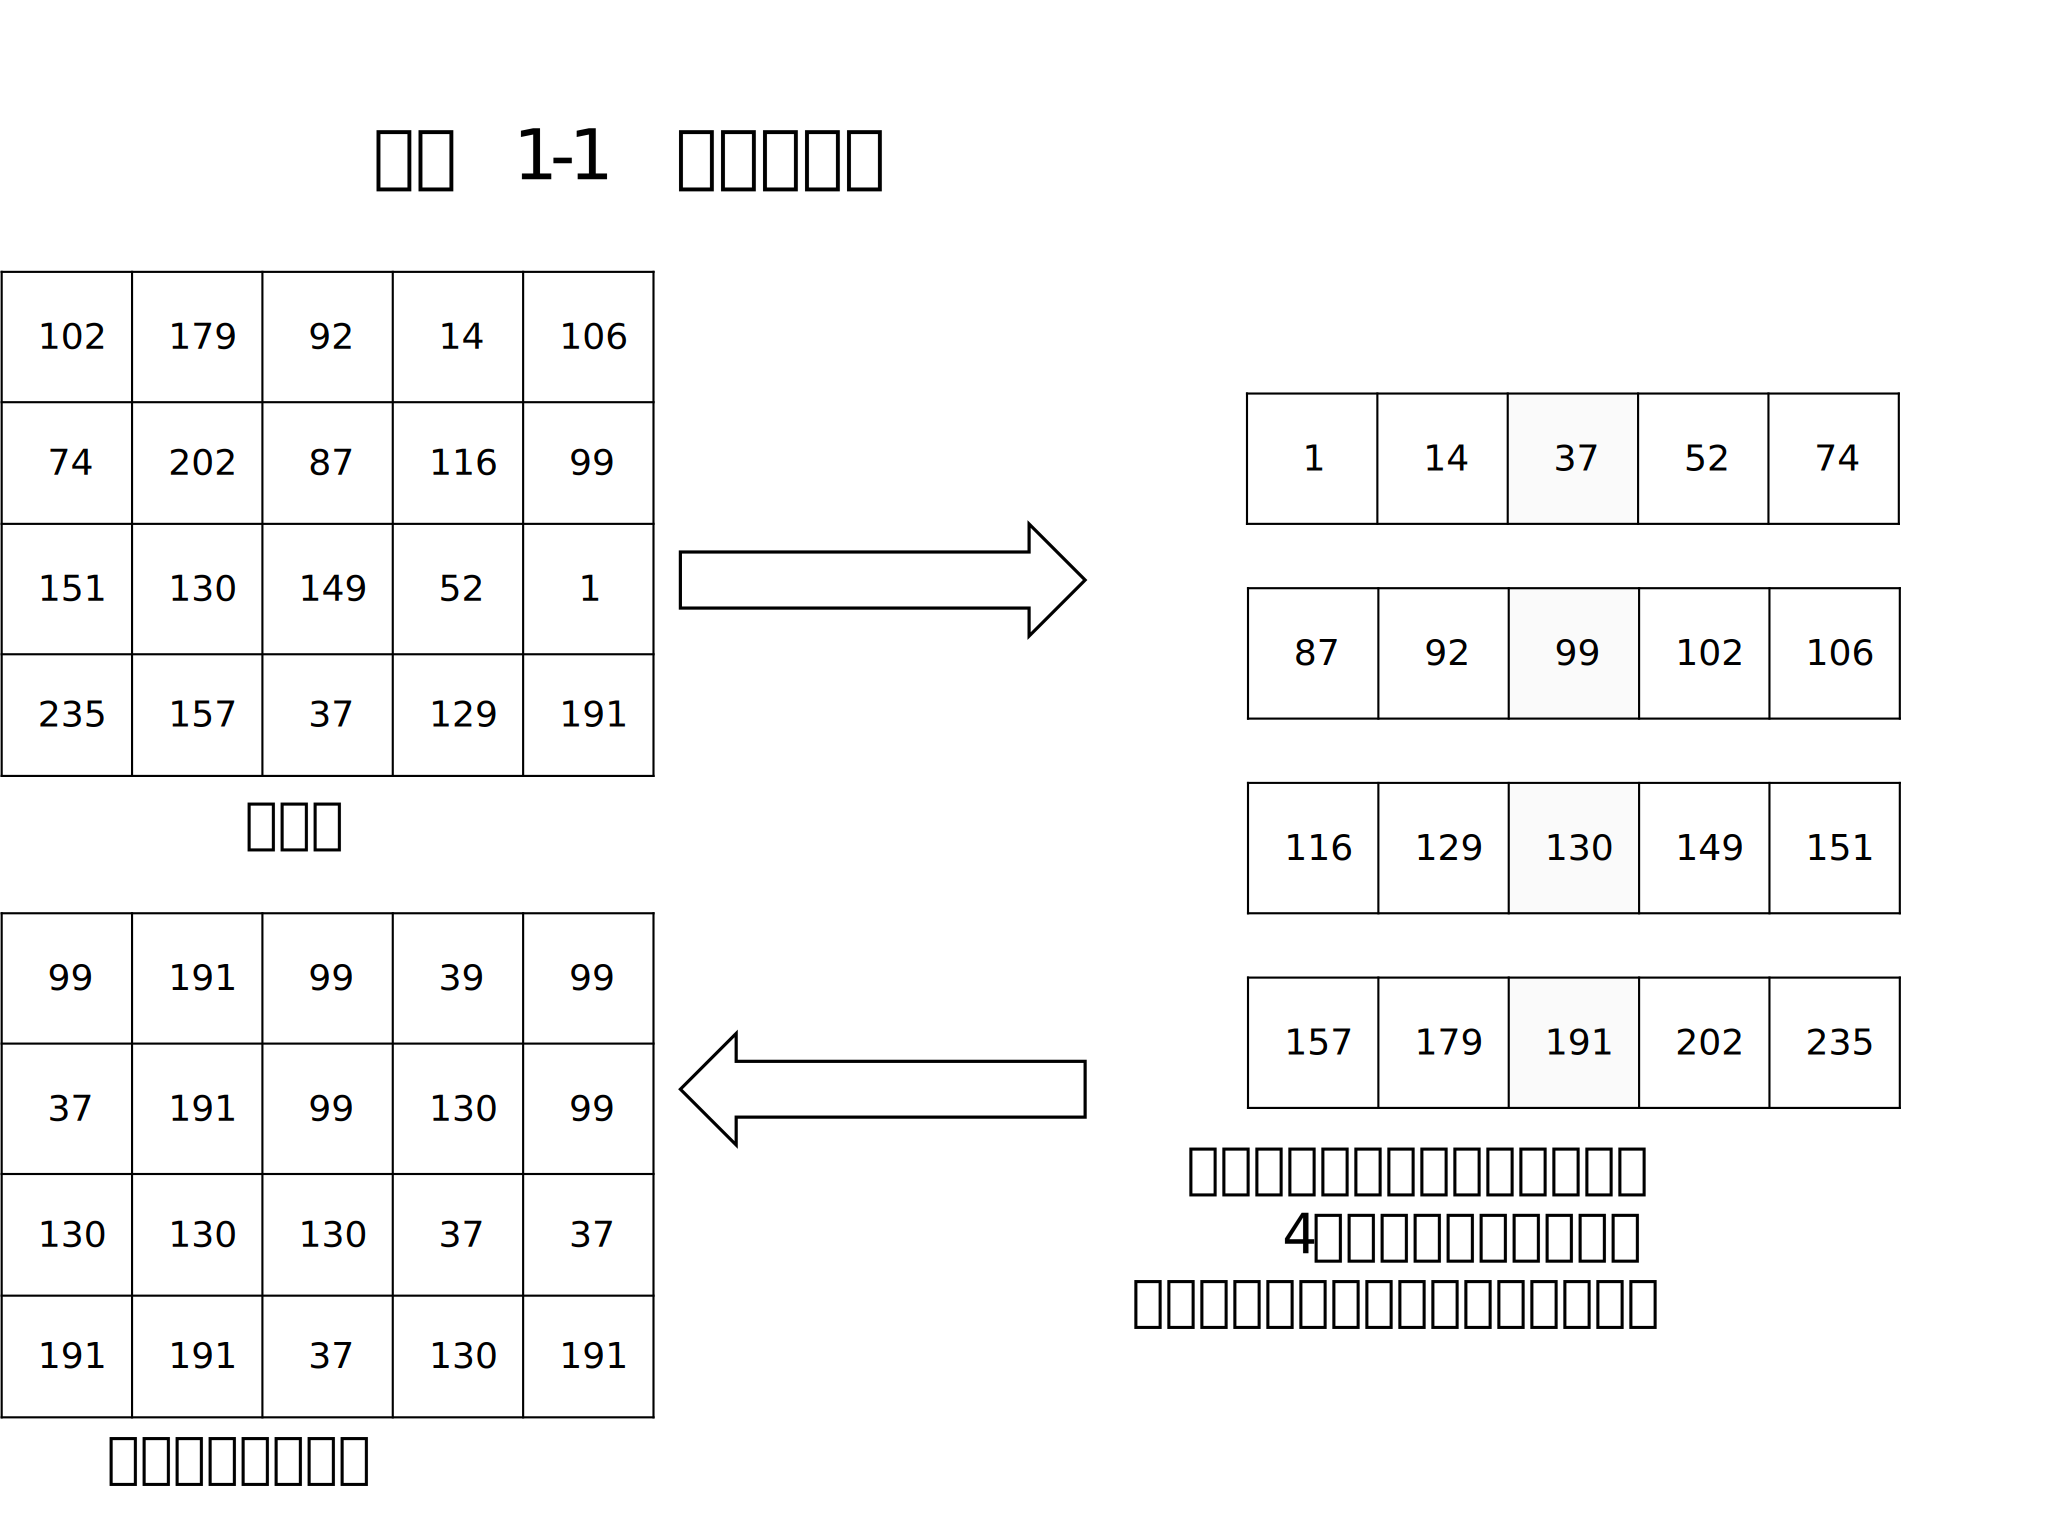
\includegraphics[width=0.85\textwidth]{問題1-1.pdf}
	\caption{メディアンカット量子化の結果}
	\label{fig:median_cut}
\end{figure}

\subsection{問題1-2: ラベリング処理}

\subsubsection{理論}
2値画像で連結成分に同一ラベルを割り当てます。2回走査法では、第1回で仮ラベル割当と等価関係記録を行い、第2回で統合します。

\subsubsection{計算・導出過程}

図A-2の10×10画素画像に対してラベリングを実行。

第1回走査では、左上から右下へ走査し、各白ピクセルについて左上・上・右上・左のピクセルを確認します。
\begin{itemize}
	\item 全て黒 → 新規ラベル割当
	\item いずれかが白 → そのラベル継承
	\item 複数が異なるラベル → 最小値割当、等価関係記録
\end{itemize}

等価ラベル関係:$A - B - C$, $E - F$, $D$

第2回走査:等価関係に基づいて代表ラベルに統一。

\begin{table}[H]
	\centering
	\begin{tabular}{|c|c|c|}
		\hline
		仮ラベル & 等価関係 & 代表ラベル \\
		\hline
		A, B, C & $A - B - C$ & A \\
		D & 単独 & D \\
		E, F & $E - F$ & E \\
		\hline
	\end{tabular}
\end{table}

\subsubsection{結果}

\begin{figure}[H]
	\centering
	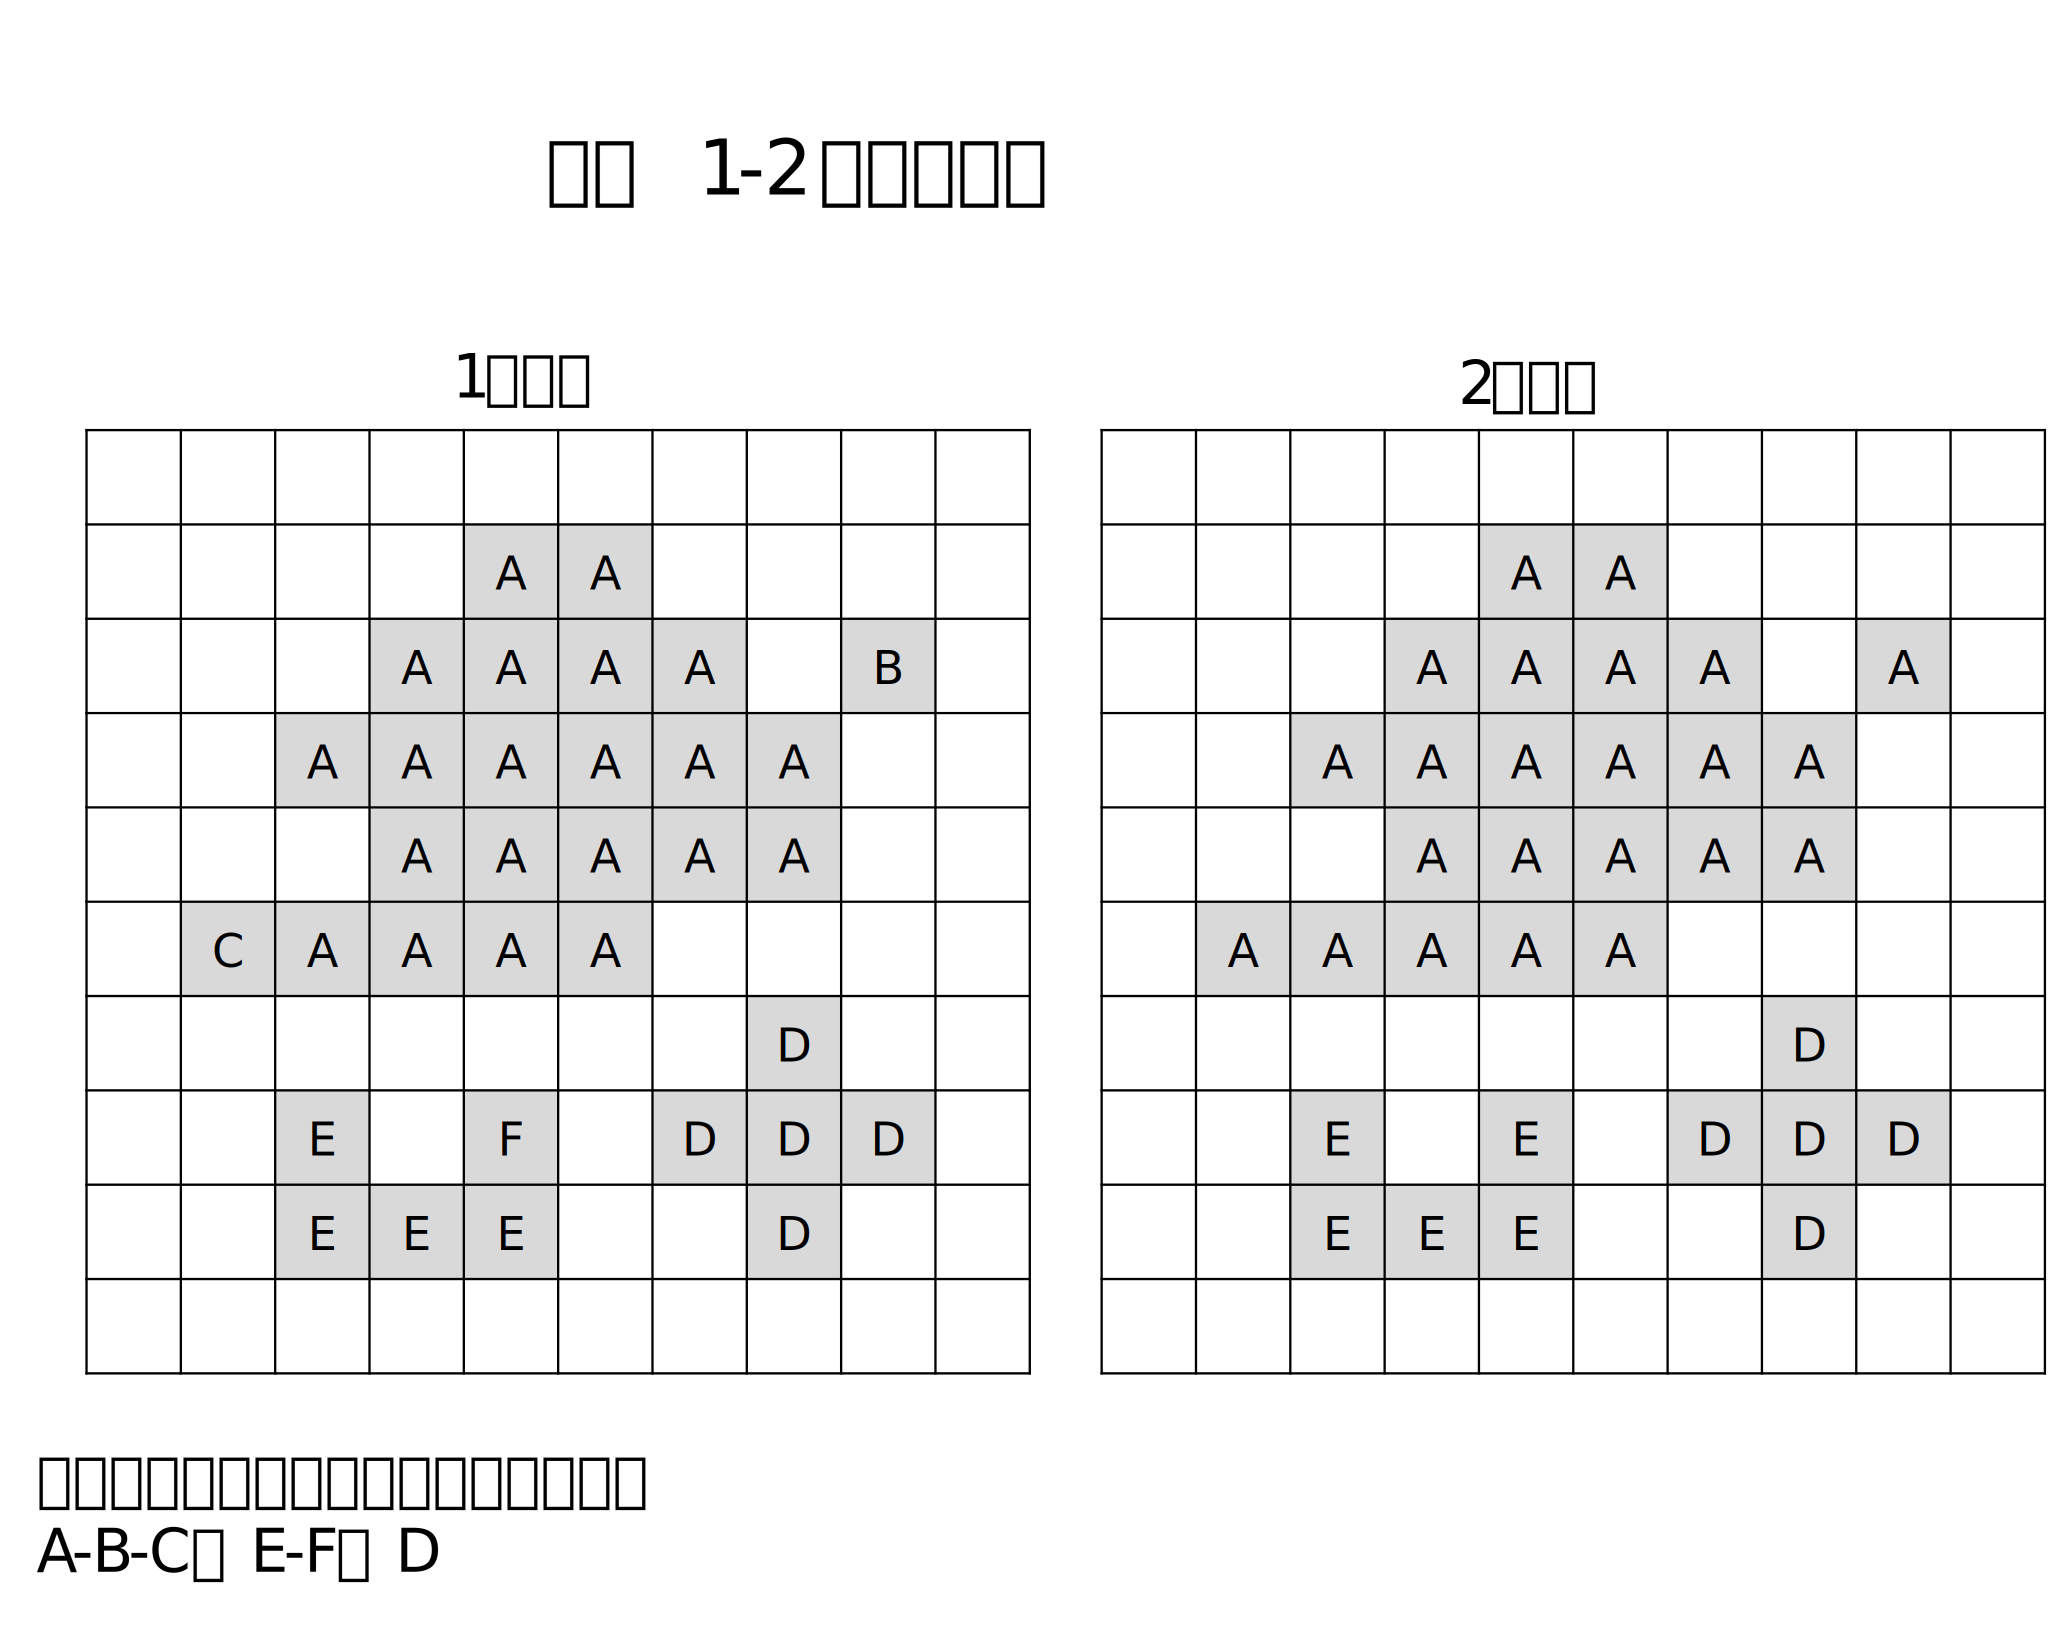
\includegraphics[width=0.9\textwidth]{問題1-2.pdf}
	\caption{ラベリング処理の結果}
	\label{fig:labeling}
\end{figure}

\subsection{問題1-3: ハフマン符号化}

\subsubsection{理論}
高確率シンボルに短い符号を割り当てる可変長符号化を行います。ハフマン木を構築することで符号を生成します。

\subsubsection{計算・導出過程}

8個のシンボルの出現確率を以下に示します。

\begin{table}[H]
	\centering
	\begin{tabular}{|c|c|c|}
		\hline
		シンボル & 確率 & 符号 \\
		\hline
		0 & 0.30 & 10 \\
		1 & 0.02 & 00001 \\
		2 & 0.06 & 0011 \\
		3 & 0.04 & 0001 \\
		4 & 0.01 & 00000 \\
		5 & 0.05 & 0010 \\
		6 & 0.20 & 01 \\
		7 & 0.32 & 11 \\
		\hline
	\end{tabular}
\end{table}

結合ステップを低い確率から順に実行すると以下の通りです。
		\begin{enumerate}
			\item 4(0.01)+1(0.02)=0.03 → A
			\item A(0.03)+3(0.04)=0.07 → B
			\item 5(0.05)+2(0.06)=0.11 → C
			\item B(0.07)+C(0.11)=0.18 → D
			\item D(0.18)+6(0.20)=0.38 → E
			\item 0(0.30)+7(0.32)=0.62 → F
			\item E(0.38)+F(0.62)=1.00 → G
		\end{enumerate}

平均符号長計算:
\begin{align*}
L &= 0.30 \times 2 + 0.02 \times 5 + 0.06 \times 4 + 0.04 \times 4 \\
  &\quad + 0.01 \times 5 + 0.05 \times 4 + 0.20 \times 2 + 0.32 \times 2 \\
  &= 2.39 \text{ ビット}
\end{align*}

等長符号(3ビット)との比較:削減量 $= 3 - 2.39 = 0.61$ ビット(約20\%削減)

\subsubsection{結果}

\begin{figure}[H]
	\centering
	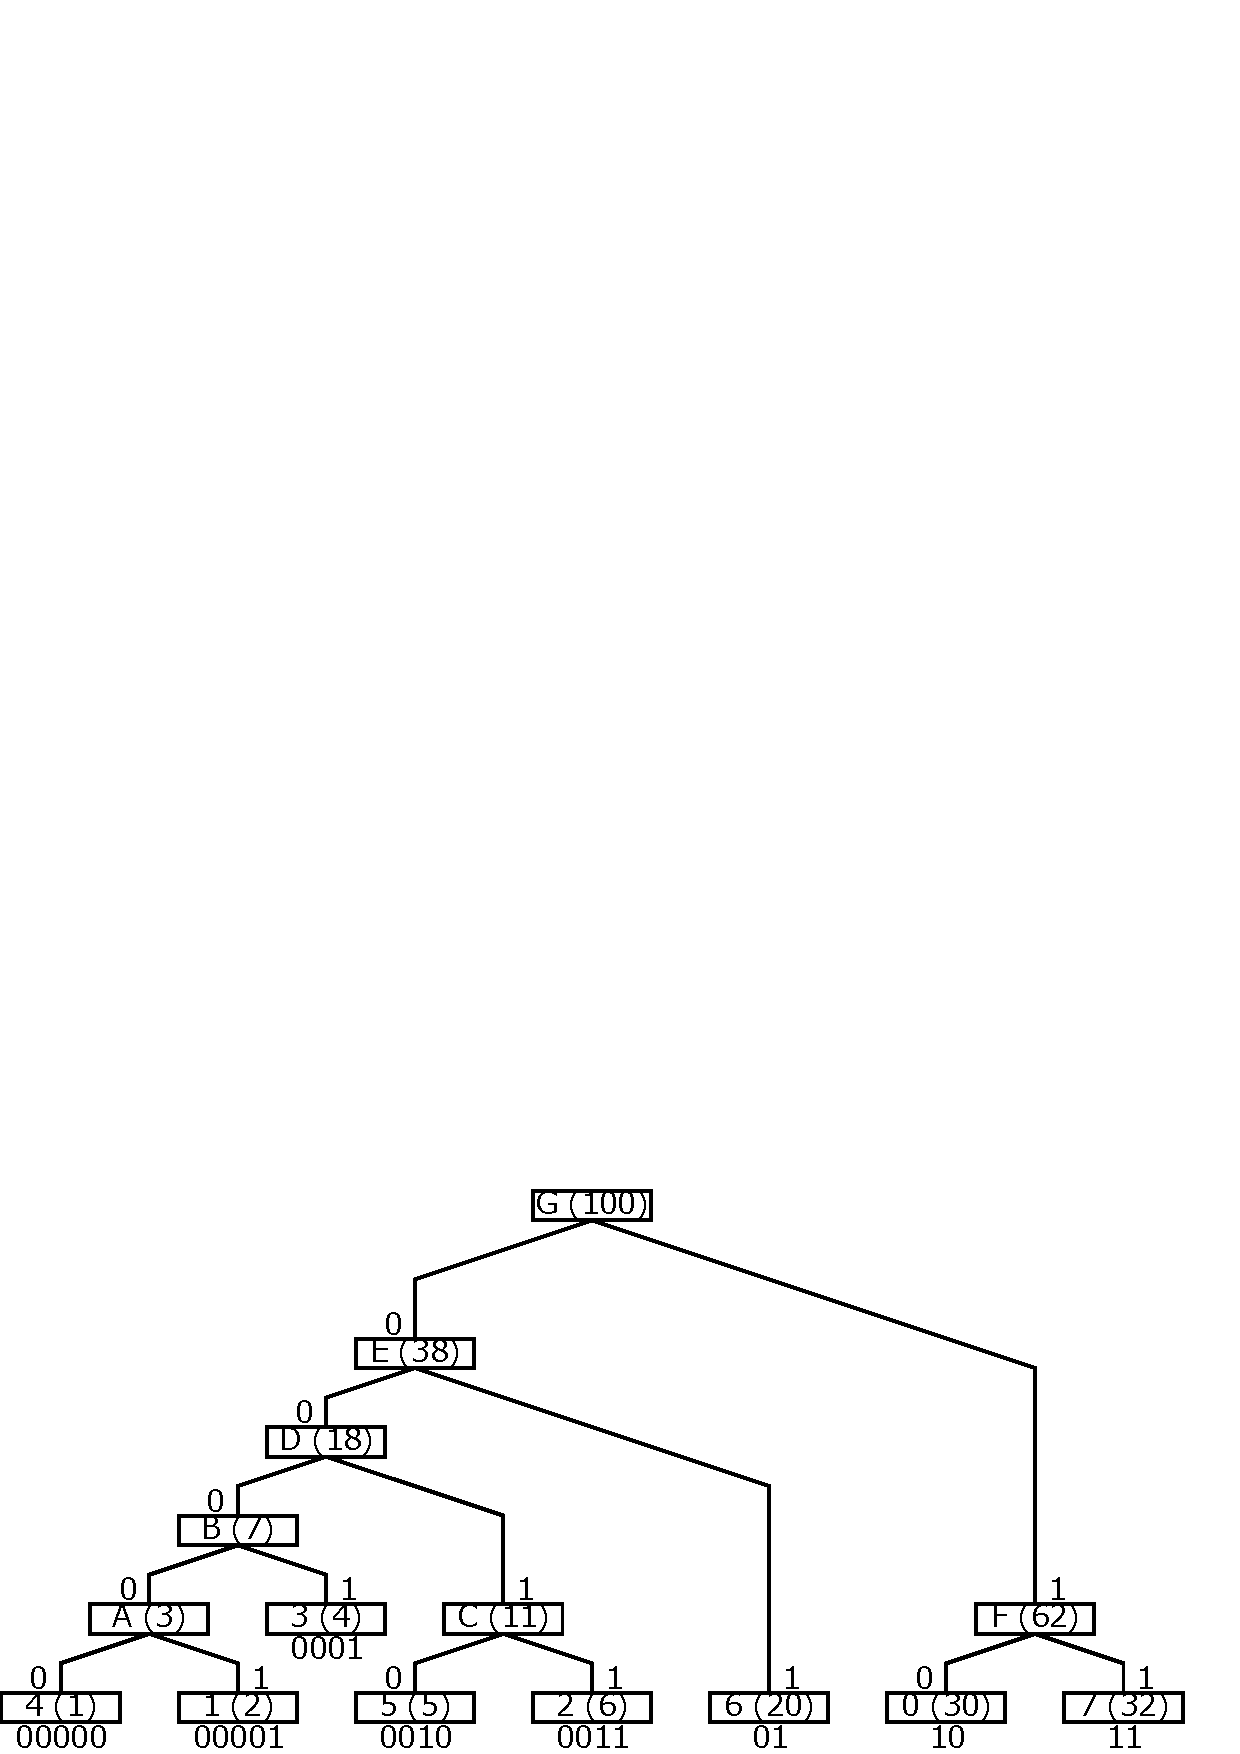
\includegraphics[width=0.8\textwidth]{問題1-3.pdf}
	\caption{ハフマン木の構造}
	\label{fig:huffman}
\end{figure}

\section{課題2}

\section{問題1: モルフォロジー処理によるノイズ除去}

\subsection{概要}
開処理と閉処理を用いてノイズを除去。

\subsubsection{理論}
開処理(収縮→膨張)で明色の孤立ノイズを除去し、閉処理(膨張→収縮)で暗色ノイズを埋める。本実装では矩形カーネルと楕円カーネルを用い、カーネルサイズ $k$ を3--15(奇数)で走査し、矩形→楕円の順で開処理を二段適用した。

\subsection{結果}
開処理(Opening = 収縮→膨張)により、白色の孤立ノイズが除去された。収縮処理で小領域が消失し、その後の膨張で主要な図形領域が復元された。本画像では白色ノイズが優勢であったため開処理を採用した。実験により、矩形構造要素(\texttt{MORPH\_RECT})は十字構造要素(\texttt{MORPH\_CROSS})よりも孤立した小ノイズの除去に有効であることが示された。実践手順として、矩形カーネルによる開処理の後に楕円形カーネル(\texttt{MORPH\_ELLIPSE})で追処理を行うことで、矩形処理後に残存する微小ノイズをさらに低減できることが確認された。矩形→楕円の順で処理を行うと形状保持と雑音除去のバランスが良好となる。閉処理(Closing = 膨張→収縮)は黒色ノイズの埋め込みに有効であるが、本課題の対象画像では適用しなかった。

\begin{figure}[H]
	\centering
	\includegraphics[width=0.95\textwidth]{problem2_1_result.png}
	\caption{Kernel size 15 での開閉処理結果(ノイズ除去後の2値画像)}
	\label{fig:morph_kernel15}
\end{figure}

	\subsubsection{考察}
	矩形→楕円の二段開処理で細粒ノイズが安定して除去できた。$k=9$ 付近がノイズ除去と形状保持の折衷点であり、$k=15$ では効果が飽和し変化が小さい。なお、黒ノイズ主体の画像に対しては閉処理の適用が有効である。

\section{問題2: JPEG品質と圧縮率の関係}

\subsection{概要}
JPEG品質と圧縮率、SSIM値の関係を調査。

\subsubsection{理論}
品質パラメータ\texttt{Q}を0--100で設定し、元PNGサイズ $S_0$ と圧縮後サイズ $S_Q$ からサイズ比 $100\times S_Q/S_0$ を算出。画質はRGBで構造類似度指数(SSIM, \texttt{win\_size}=3, \texttt{channel\_axis}=2, \texttt{data\_range}=255)を評価した。

\subsection{結果}
下表は本レポートで得られた数値(品質Q、サイズ比、SSIM)を整理したもの。

\begin{table}[H]
\centering
\caption{品質Qによるサイズ比とSSIM}
\label{tab:jpeg_q_ssim}
\begin{tabular}{rcc}
\toprule
Q & サイズ比(\%) & SSIM \\
\midrule
0   & 0.9  & 0.327 \\
10  & 2.2  & 0.520 \\
20  & 3.6  & 0.609 \\
30  & 4.8  & 0.656 \\
40  & 5.8  & 0.686 \\
50  & 6.7  & 0.709 \\
60  & 7.7  & 0.729 \\
70  & 9.3  & 0.753 \\
80  & 11.8 & 0.783 \\
90  & 17.7 & 0.825 \\
100 & 45.5 & 0.871 \\
\bottomrule
\end{tabular}
\end{table}

\begin{figure}[H]
\centering
\includegraphics[width=0.95\textwidth]{problem2_2_result.png}
\caption{JPEG品質Qごとの視覚比較とサイズ比・SSIM(提示画像)}
\label{fig:jpeg_q_grid}
\end{figure}

\subsubsection{考察}
SSIMはQに単調増加し、\textbf{Q=80}で0.783、\textbf{Q=90}で0.825となるがサイズ比は11.8\%→17.7\%へ増加する。視覚・数値の両面から実用的には\textbf{Q=80~90}が現実的で、\textbf{Q=100}は45.5\%まで肥大し利得が小さい。容量重視なら\textbf{Q=10}(サイズ比2.2\%、SSIM 0.520)も用途次第で許容される。

\section{問題3: 2次元FFTと振幅スペクトル}

\subsection{概要}
グレースケール画像を2次元FFTで周波数領域に変換し、振幅スペクトルを分析。

\subsubsection{理論}
各入力画像を中心から最大の正方形にトリミングし、2次元FFT後に\texttt{fftshift}で低周波を中心化。振幅スペクトルは $20\log_{10}(|F|+1)$ の対数スケールで可視化した。

\subsection{結果}

\begin{figure}[H]
\centering
\includegraphics[width=0.85\textwidth]{problem2_3_result.png}
\caption{グレースケール画像の2次元振幅スペクトル(中央化)}
\label{fig:fft_magnitude}
\end{figure}

\begin{figure}[H]
\centering
\begin{minipage}{0.48\textwidth}
  \centering
  \includegraphics[width=\linewidth]{problem2_3_result_0.png}
  \vspace{1mm}
  \small (a) 入力画像1の振幅スペクトル
\end{minipage}\hfill
\begin{minipage}{0.48\textwidth}
  \centering
  \includegraphics[width=\linewidth]{problem2_3_result_1.png}
  \vspace{1mm}
  \small (b) 入力画像2の振幅スペクトル
\end{minipage}

\vspace{6pt}

\begin{minipage}{0.48\textwidth}
  \centering
  \includegraphics[width=\linewidth]{problem2_3_result_2.png}
  \vspace{1mm}
  \small (c) 入力画像3の振幅スペクトル
\end{minipage}\hfill
\begin{minipage}{0.48\textwidth}
  \centering
  \includegraphics[width=\linewidth]{problem2_3_result_3.png}
  \vspace{1mm}
  \small (d) 入力画像4の振幅スペクトル
\end{minipage}

\vspace{6pt}

\begin{center}
  \begin{minipage}{0.48\textwidth}
    \centering
    \includegraphics[width=\linewidth]{problem2_3_result_4.png}
    \vspace{1mm}
    \small (e) 入力画像5の振幅スペクトル
  \end{minipage}
\end{center}
\caption{同一の2次元FFT処理を別入力画像に適用した結果(左上→右下: (a)〜(e))。}
\label{fig:fft_magnitude_multi}
\end{figure}

\noindent 図\ref{fig:fft_magnitude_multi}は、図\ref{fig:fft_magnitude}と同一の処理を別入力画像に適用した結果である。各サブ図はそれぞれ異なる入力画像に対する結果を示す。

\subsubsection{考察}
周期性の強い幾何パターンでは明瞭な格子状ピークが現れ、細かい線描は高周波まで広がるスペクトルとなった。自然テクスチャはエネルギーが中心寄りに分布し、モアレ風パターンでは対角方向のピークが強調された。

% 考察は本問題では省略します。

\paragraph{画像タイプ別プロンプト例}
今回のレポートで示した、特に問題2-3で処理対象とした入力画像は、以下に示すプロンプトを用いてNanoBananaProで生成したものです。

\begin{description}
\item[パターン1:幾何学的・周期的な構造] \hfill \\
\textbf{Prompt:}
\begin{quote}\texttt{Hyper-intricate kaleidoscope pattern, complex geometric fractal, high contrast black and white, mathematical symmetry, sharp edges, detailed mandala, optical illusion art, 8k resolution --ar 1:1}\end{quote}

\item[パターン2:細かい線描・版画調] \hfill \\
\textbf{Prompt:}
\begin{quote}\texttt{Detailed cross-hatching illustration in the style of Gustave Dor\'e, antique etching of a dense forest, intricate ink lines, engraving style, high detail, sharp texture, masterpiece --ar 1:1}\end{quote}

\item[パターン3:人工的なグリッド・都市・回路] \hfill \\
\textbf{Prompt:}
\begin{quote}\texttt{Aerial top-down view of a futuristic cyber city, dense skyscrapers, intricate circuit board texture, metallic surfaces, high contrast, greeble details, sci-fi architecture, sharp focus --ar 1:1}\end{quote}

\item[パターン4:自然界のランダムなテクスチャ] \hfill \\
\textbf{Prompt:}
\begin{quote}\texttt{Macro photography of intricate bird feathers, extreme close-up of insect wing texture, biological cells patterns, fibrous texture, sharp details, high texture quality, monochrome photography --ar 1:1}\end{quote}

\item[パターン5:ハーフトーン・モアレ(ドット)] \hfill \\
\textbf{Prompt:}
\begin{quote}
\raggedright\ttfamily
Halftone dot pattern portrait, pop art style, comic book shading, distinct dots, moire pattern effect, glitch art, high contrast, monochrome --ar 1:1
\end{quote}
\end{description}

\paragraph{生成時のコツ}
\begin{itemize}
\item "Intricate"、"Detailed"、"Dense"、"High contrast" といった語を含めると、周波数的に特徴が出やすくなる。
\item コントラストを高めるとエッジ成分が強調され、FFT結果が見やすくなる。
\end{itemize}

\section{問題4: 周波数フィルタの応用}

\subsection{概要}
理想的ローパスフィルタ(ILPF)とガウシアンハイパスフィルタ(GHPF)を、カットオフ周波数 $D_0$ を 10/30/60 と変化させ適用し、効果を比較。

\subsubsection{理論}
ILPFは周波数距離 $D\le D_0$ を1、その他を0とするマスク $H_{\mathrm{ILPF}}(D)$ を掛ける。GHPFは $H_{\mathrm{GHPF}}(D)=1-\exp\{-D^2/(2D_0^2)\}$ で低周波を抑圧し高周波を通過させる。いずれも\texttt{fftshift}後の周波数平面でマスクを乗算し、逆FFTで復元した。

\subsection{結果}

\begin{figure}[H]
\centering
\includegraphics[width=0.95\textwidth]{problem2_4_result.png}
\caption{ローパスフィルタとハイパスフィルタの適用結果比較(代表例)}
\label{fig:filter_comparison}
\end{figure}

\begin{figure}[H]
\centering
\begin{minipage}{0.48\textwidth}
  \centering
  \includegraphics[width=\linewidth]{problem2_4_result_0.png}
  \vspace{1mm}
  \small (a) 入力画像1の比較
\end{minipage}\hfill
\begin{minipage}{0.48\textwidth}
  \centering
  \includegraphics[width=\linewidth]{problem2_4_result_1.png}
  \vspace{1mm}
  \small (b) 入力画像2の比較
\end{minipage}

\vspace{6pt}

\begin{minipage}{0.48\textwidth}
  \centering
  \includegraphics[width=\linewidth]{problem2_4_result_2.png}
  \vspace{1mm}
  \small (c) 入力画像3の比較
\end{minipage}\hfill
\begin{minipage}{0.48\textwidth}
  \centering
  \includegraphics[width=\linewidth]{problem2_4_result_3.png}
  \vspace{1mm}
  \small (d) 入力画像4の比較
\end{minipage}

\vspace{6pt}

\begin{center}
  \begin{minipage}{0.48\textwidth}
    \centering
    \includegraphics[width=\linewidth]{problem2_4_result_4.png}
    \vspace{1mm}
    \small (e) 入力画像5の比較
  \end{minipage}
\end{center}
\caption{同一のフィルタ処理を別入力画像で試した結果(左上→右下: (a)〜(e))。}
\label{fig:filter_results_multi}
\end{figure}

\noindent 図\ref{fig:filter_results_multi}は、図\ref{fig:filter_comparison}と同一の処理を別入力画像に適用した結果である。各サブ図に示したカットオフ周波数 $D_0$ はサブキャプション((a)~(e))に記載してある。

\textbf{ローパスフィルタ(ILPF)}: 低周波成分のみを通し、高周波(ノイズ・細部)を除去。結果は全体的にぼかされ、目や顔の大型構造は保持される一方、毛並みなどの細かいテクスチャは消失。ノイズ除去やスムージングに有効。

\textbf{ハイパスフィルタ(GHPF)}: DC成分と低周波を除去し、高周波のみを通す。結果はエッジが明るく浮き出ち、目・口・毛並みなどの細部が強調される。大きな領域は暗くなり、画像全体はコントラストが低下。エッジ検出と細部抽出に有効。

\textbf{カットオフ周波数D0の影響}: D0を10/30/60と変化させた結果、D0が小さいほど通過する周波数帯域が狭まる。ローパスではD0=10で極端なぼかし効果、D0=60で細部を一定程度保持する。ハイパスではD0=10でエッジ成分のみが抽出され、D0=60では中間周波数も強調されより豊かなテクスチャが得られた。D0の選択は目的(ノイズ除去vs細部保持)に応じて調整すべきである。

\subsubsection{考察}
ILPFはD0=10で強いぼかしとなり輪郭も鈍化、D0=60で顔や毛並みの細部が残る。GHPFはD0=10でエッジ抽出的になり暗部が増えるが、D0=60では中間周波も残り質感強調が得られた。目的がノイズ除去なら小さめ、質感強調なら大きめのD0が適切。

\clearpage

\section*{付録: プログラムリスト}

\subsection*{問題1: モルフォロジー処理}

\lstinputlisting[caption={問題1 モルフォロジー処理によるノイズ除去}, label={lst:code1}, language=Python]{../問題2_1.py}

\clearpage

\subsection*{問題2: JPEG品質と圧縮率}

\lstinputlisting[caption={問題2 JPEG品質と圧縮率の関係調査}, label={lst:code2}, language=Python]{../問題2_2.py}

\clearpage

\subsection*{問題3: 2次元FFTと振幅スペクトル}

\lstinputlisting[caption={問題3 2次元FFTと振幅スペクトル}, label={lst:code3}, language=Python]{../問題2_3.py}

\clearpage

\subsection*{問題4: 周波数フィルタの応用}

\lstinputlisting[caption={問題4 周波数フィルタの応用}, label={lst:code4}, language=Python]{../問題2_4.py}

\end{document}
